% Tasks:
% Put in estimate of galactic NH (Moritz)
% Dickey and Lockman, 1990, Annu. Rev. Astron. Astrophys., 28, 215
% get: 1.73 e20 - maybe plot second model with nh fixed? - plot done, but not yet included
% Get TESS lightcurve to check for variability (MMax)
% Is a jet reasonable (eqn 6) (Moritz to put some numbers in)
% Arcus simulations (Moritz)
% Check if X-East and X-West coincide with GAIA sources (i.e. they are foreground stars) - good hint from Christian (Moritz) - done. No GAIA DR2 or 2MASS sources are close to X-East and X-North.
% Consolidate discussion on shock physics - mostly done
% discuss variability and magnetic field
% plot of L_X / L_bol for some classes of objects. What's the other axis? rosby number? Age? Period?



%% using aastex version 6.3
\documentclass[linenumbers]{aastex631}
\usepackage{amsmath}
\usepackage{amssymb}

\newcommand{\be}{\begin{equation}}
\newcommand{\ee}{\end{equation}}

%% The default is a single spaced, 10 point font, single spaced article.
%% There are 5 other style options available via an optional argument. They
%% can be invoked like this:
%%
%% \documentclass[arguments]{aastex631}
%%
%% where the layout options are:
%%
%%  twocolumn   : two text columns, 10 point font, single spaced article.
%%                This is the most compact and represent the final published
%%                derived PDF copy of the accepted manuscript from the publisher
%%  manuscript  : one text column, 12 point font, double spaced article.
%%  preprint    : one text column, 12 point font, single spaced article.
%%  preprint2   : two text columns, 12 point font, single spaced article.
%%  modern      : a stylish, single text column, 12 point font, article with
%% 		  wider left and right margins. This uses the Daniel
%% 		  Foreman-Mackey and David Hogg design.
%%  RNAAS       : Supresses an abstract. Originally for RNAAS manuscripts
%%                but now that abstracts are required this is obsolete for
%%                AAS Journals. Authors might need it for other reasons. DO NOT
%%                use \begin{abstract} and \end{abstract} with this style.
%%
%% Note that you can submit to the AAS Journals in any of these 6 styles.
%%
%% There are other optional arguments one can invoke to allow other stylistic
%% actions. The available options are:
%%
%%   astrosymb    : Loads Astrosymb font and define \astrocommands.
%%   tighten      : Makes baselineskip slightly smaller, only works with
%%                  the twocolumn substyle.
%%   times        : uses times font instead of the default
%%   linenumbers  : turn on lineno package.
%%   trackchanges : required to see the revision mark up and print its output
%%   longauthor   : Do not use the more compressed footnote style (default) for
%%                  the author/collaboration/affiliations. Instead print all
%%                  affiliation information after each name. Creates a much
%%                  longer author list but may be desirable for short
%%                  author papers.
%% twocolappendix : make 2 column appendix.
%%   anonymous    : Do not show the authors, affiliations and acknowledgments
%%                  for dual anonymous review.
%%
%% these can be used in any combination, e.g.
%%
%% \documentclass[twocolumn,linenumbers,trackchanges]{aastex631}
%%
%% AASTeX v6.* now includes \hyperref support. While we have built in specific
%% defaults into the classfile you can manually override them with the
%% \hypersetup command. For example,
%%
%% \hypersetup{linkcolor=red,citecolor=green,filecolor=cyan,urlcolor=magenta}
%%
%% will change the color of the internal links to red, the links to the
%% bibliography to green, the file links to cyan, and the external links to
%% magenta. Additional information on \hyperref options can be found here:
%% https://www.tug.org/applications/hyperref/manual.html#x1-40003
%%
%% Note that in v6.3 "bookmarks" has been changed to "true" in hyperref
%% to improve the accessibility of the compiled pdf file.
%%
%% If you want to create your own macros, you can do so
%% using \newcommand. Your macros should appear before
%% the \begin{document} command.
%%

%% Reintroduced the \received and \accepted commands from AASTeX v5.2
%\received{March 1, 2021}
%\revised{April 1, 2021}
%\accepted{\today}

%% Command to document which AAS Journal the manuscript was submitted to.
%% Adds "Submitted to " the argument.
%\submitjournal{PSJ}

%%
%% For manuscript without any need to use \collaboration the
%% \AuthorCollaborationLimit command from v6.2 can still be used to
%% show a subset of authors.
%
%\AuthorCollaborationLimit=2
%
%% will only show Schwarz & Muench on the front page of the manuscript
%% (assuming the \collaboration and \nocollaboration commands are
%% commented out).
%%
%% Note that all of the author will be shown in the published article.
%% This feature is meant to be used prior to acceptance to make the
%% front end of a long author article more manageable. Please do not use
%% this functionality for manuscripts with less than 20 authors. Conversely,
%% please do use this when the number of authors exceeds 40.
%%
%% Use \allauthors at the manuscript end to show the full author list.
%% This command should only be used with \AuthorCollaborationLimit is used.

%% The following command can be used to set the latex table counters.  It
%% is needed in this document because it uses a mix of latex tabular and
%% AASTeX deluxetables.  In general it should not be needed.
%\setcounter{table}{1}

%%%%%%%%%%%%%%%%%%%%%%%%%%%%%%%%%%%%%%%%%%%%%%%%%%%%%%%%%%%%%%%%%%%%%%%%%%%%%%%%
%%
%% The following section outlines numerous optional output that
%% can be displayed in the front matter or as running meta-data.
%%
%% If you wish, you may supply running head information, although
%% this information may be modified by the editorial offices.
\shorttitle{X-ray emission from TYC 2597-735-1}
\shortauthors{G\"unther et al.}

\graphicspath{{./}{figures/}}
%% This is the end of the preamble.  Indicate the beginning of the
%% manuscript itself with \begin{document}.

\begin{document}

\title{X-ray emission from TYC 2597-735-1}

%% LaTeX will automatically break titles if they run longer than
%% one line. However, you may use \\ to force a line break if
%% you desire. In v6.31 you can include a footnote in the title.

%% A significant change from earlier AASTEX versions is in the structure for
%% calling author and affiliations. The change was necessary to implement
%% auto-indexing of affiliations which prior was a manual process that could
%% easily be tedious in large author manuscripts.
%%
%% The \author command is the same as before except it now takes an optional
%% argument which is the 16 digit ORCID. The syntax is:
%% \author[xxxx-xxxx-xxxx-xxxx]{Author Name}
%%
%% This will hyperlink the author name to the author's ORCID page. Note that
%% during compilation, LaTeX will do some limited checking of the format of
%% the ID to make sure it is valid. If the "orcid-ID.png" image file is
%% present or in the LaTeX pathway, the OrcID icon will appear next to
%% the authors name.
%%
%% Use \affiliation for affiliation information. The old \affil is now aliased
%% to \affiliation. AASTeX v6.31 will automatically index these in the header.
%% When a duplicate is found its index will be the same as its previous entry.
%%
%% Note that \altaffilmark and \altaffiltext have been removed and thus
%% can not be used to document secondary affiliations. If they are used latex
%% will issue a specific error message and quit. Please use multiple
%% \affiliation calls for to document more than one affiliation.
%%
%% The new \altaffiliation can be used to indicate some secondary information
%% such as fellowships. This command produces a non-numeric footnote that is
%% set away from the numeric \affiliation footnotes.  NOTE that if an
%% \altaffiliation command is used it must come BEFORE the \affiliation call,
%% right after the \author command, in order to place the footnotes in
%% the proper location.
%%
%% Use \email to set provide email addresses. Each \email will appear on its
%% own line so you can put multiple email address in one \email call. A new
%% \correspondingauthor command is available in V6.31 to identify the
%% corresponding author of the manuscript. It is the author's responsibility
%% to make sure this name is also in the author list.
%%
%% While authors can be grouped inside the same \author and \affiliation
%% commands it is better to have a single author for each. This allows for
%% one to exploit all the new benefits and should make book-keeping easier.
%%
%% If done correctly the peer review system will be able to
%% automatically put the author and affiliation information from the manuscript
%% and save the corresponding author the trouble of entering it by hand.


\author[0000-0003-4243-2840]{Hans Moritz G{\"u}nther}
\affiliation{MIT Kavli Institute for Astrophysics and Space Research, 77 Massachusetts Avenue, Cambridge, MA 02139, USA}
\author{Keri Hoadley}
\affiliation{The University of Iowa, Dept. of Physics \& Astronomy, Van Allen Hall, Iowa City, IA, 52242, USA}
\affiliation{California Institute of Technology, Dept. of Physics, Mathematics, and Astronomy, Cahill Center for Astronomy \& Astrophysics, Pasadena, CA 91125, USA}
\author{Brian D.~Metzger}
\affiliation{Columbia Astrophysics Laboratory, Columbia University}
\author{Ken Shen}
\affiliation{author ordering will be decided later}
\author{Maximilian N. G{\"u}nther}
\affiliation{Department of Physics, and Kavli Institute for Astrophysics and Space Research, Massachusetts Institute of Technology, 77 Massachusetts Avenue, Cambridge, MA 02139, US}
\affiliation{Juan Carlos Torres Fellow}
\author{Your name here}
\affiliation{author ordering will be decided later}

%% Note that the \and command from previous versions of AASTeX is now
%% depreciated in this version as it is no longer necessary. AASTeX
%% automatically takes care of all commas and "and"s between authors names.

%% AASTeX 6.31 has the new \collaboration and \nocollaboration commands to
%% provide the collaboration status of a group of authors. These commands
%% can be used either before or after the list of corresponding authors. The
%% argument for \collaboration is the collaboration identifier. Authors are
%% encouraged to surround collaboration identifiers with ()s. The
%% \nocollaboration command takes no argument and exists to indicate that
%% the nearby authors are not part of surrounding collaborations.

%% Mark off the abstract in the ``abstract'' environment.
\begin{abstract}
abstract here

\end{abstract}

%% Keywords should appear after the \end{abstract} command.
%% The AAS Journals now uses Unified Astronomy Thesaurus concepts:
%% https://astrothesaurus.org
%% You will be asked to selected these concepts during the submission process
%% but this old "keyword" functionality is maintained in case authors want
%% to include these concepts in their preprints.
\keywords{}


\section{Introduction} \label{sec:intro}
%%%% Old intro
% Binary and multi-star systems make up an appreciable percentage the star systems in the Galaxy \citep{Raghavan+2010}. It is no surprise, then, that eventually, closely orbiting binary stars may interact through events that exchange and shed matter from one star to another (e.g., common envelope evolution (CEE); \citealt{}) or end with the complete engulfment of one star by another (e.g., \citealt{}). This exchange of matter and energy between stars in close orbit with one another leads not only to drastic consequences on the evolutionary properties of the system (e.g., the formation of an accretion disk; \citealt{}), but to dramatic changes in the properties of the stars themselves.

% In the case of a complete stellar merger event, the engulfment process adds a significant amount of energy into the consuming star (E$>$XXX; \citealt{}), throwing its atmosphere and interior our of equilibrium and leading to the production of enlarged convective regions, elevated levels of magnetic activity, stellar envelope inflation, and a spin-up in stellar rotation rate \citep{}. Outflows and jets of appreciable speeds ($v>$100's km/s), powered by the stellar collision itself, contaminates the intervening space with quick-forming dust, molecules, and gas \citep{}. Over time, these outflows sweep up and build up appreciable mass, initiating interstellar shocks that change the energetic properties of interstellar material around them and potentially destroying the dust-rich matter formed as the outflow cooled away from its stellar merger origins.

% % What is the motivation to look in for X-ray signals?
% A key gap in our knowledge about stellar merger processes and long-term impacts on the outcomes of their stellar properties and systems is whether stellar collisions, whether grazing or direct, ignites or enhances magnetic activity on the impacted star(s). Stellar magnetic fields, if present, influence almost every aspect of their environments. Magnetic coupling to surrounding dust and gas left bound in orbit around the stellar merger remnant leads to accretion onto the star, providing a source of material to replenish the star(s) and leading to elevated levels of high energy radiation, in the form of line and continuum emissions, spanning the UV to the X-ray \citep{}. These increased levels of radiations further impact the stellar environment, ionizing particles and leading to changes in chemistry of the circumstellar disk over time. Magnetorotational accretion may lead to sustained outflows and jets, pumping more material to the surrounding ISM \citep{}. In other astrophysical accretion disks, stellar magnetic fields play a key role in the dispersion of the disks, defining their expected lifetimes and impact on the final properties of the stellar system \citep{}.


%%%% New intro: Outline
%% 1. TYC and BRN discovery as recent (1000's years old) stellar merger event
%% 2. Prime laboratory to test and explore theorized behaviors and evolution of such systems
%% 3. Serendipitous discovery of X-ray emission by Chandra begs the question: what is generating this high energy radiation both in the BRN and near TYC?
%% 4. Outline of study
Binary and multi-star systems make up over 1/3 of the star systems in the Galaxy \citep{Raghavan+2010}. It is no surprise, then, that eventually, closely orbiting binary stars may interact through events that exchange and shed matter from one star to another (e.g., common envelope evolution (CEE)) or end with the complete engulfment of one star by another (e.g., \citealt{Ivanova+2013}). TYC 2597-735-1 is one of only a few examples of a recent ($t \sim$ 2,000 - 5,000 years ago), unobscured (E(B-V) $\sim$ 0.02) stellar merger remnant found to date \citep{2020Natur.587..387H}. This makes TYC 2597-735-1 a rare astrophysical laboratory where we can test physical models of stellar merger behaviors, characteristics, and long-term evolution.

One key stellar behavioral shift that may rise as a result of a stellar merger is the generation of a strong magnetic field \citep{Schneider+2016}. Roughly 10\% of intermediate- to high-mass stars ($M_{\star} \gtrsim$ 1.5 $M_{\odot}$) have strong magnetic fields, whose origins are currently unknown (e.g., \citealt{Donati+2009,Fossati+2015,Grunhut+2017}). \citet{Soker&Tylenda2007} showed that the extended envelope of a merger product may host a large convective region. Paired with a rapid rotation rate, an efficient dynamo may result, giving rise to strong magnetic activity. The presence of magnetic fields has strong implications on the long-term evolution of the stellar merger system. For example, magnetic fields may drive magnetorotational accretion of surrounding material, help slow down rapidly rotating stars via magnetic breaking, and power jets (e.g., \citealt{Schneider+2020}). All these mechanisms, over long timescales, have consequences on the final outcome of a stellar merger remnant as it settles to its equilibrium state.

\citet{Soker&Tylenda2007} suggest the strongest magnetic activity tied to a stellar merger's revitalized dynamo may last centuries. Recent suspected stellar mergers (like red luminous novae) are obscured from view by outflows ejected during the merger event itself (e.g., \citealt{Bond+2003, Tylenda+2016}). TYC 2597-735-1 shows evidence that it harbors a persisting, strong magnetic field \citep[e.g., H$\alpha$ emission and variability, radial velocity shifts strongly correlated with the Ca II IRT stellar atmospheric features][]{2020Natur.587..387H}. One way to test whether its hypothetical magnetic field exists is to look for signs of X-ray emission at TYC 2597-735-1 and compare its luminosity to the remnant's bolometric luminosity \citep{Soker&Tylenda2007}.

<<<<<<< HEAD
TYC 2597-735-1 and the last vestiges of its dissolving outflow, the ``Blue Ring Nebula'' (BRN; \citealt{2020Natur.587..387H}), were partially observed by chance with Chandra over a decade ago. Here, we report the findings of this serendipitous \emph{Chandra} observation and present a new \emph{TESS} lightcurve. We explore whether the X-ray emission observed at TYC 2597-735-1 is consistent with dynamo-driven magnetic field activity or other sources near the star. We summarize the stellar properties of TYC 2597-735-1 in Section~\ref{sec:properties}. In Section~\ref{sec:data}, we describe the observations, the source detection methods implemented to retrieve X-ray signal from regions in the BRN and around TYC 2597-735-1 and the X-ray properties of these regions. In Section~\ref{sec:discussion}, we explore different physical mechanisms that may explain the X-ray luminosity and spectral characteristics observed for TYC 2597-735-1 and place physical limits on the properties of the BRN shock region from its X-ray diagnostics. We conclude in Section~\ref{sec:summary} with a summary and describe prospects for future observations.
=======
TYC 2597-735-1 and the last vestiges of its dissolving outflow, the ``Blue Ring Nebula'' (BRN; \citealt{2020Natur.587..387H}), were partially observed by chance with Chandra over a decade ago. Here, we report the findings of this serendipitous \emph{Chandra} observation and present a new \emph{TESS} lightcurve. We explore whether the X-ray emission observed at TYC 2597-735-1 is consistent with dynamo-driven magnetic field activity or other sources near the star. We summarize the stellar properties of TYC 2597-735-1 in Section~\ref{sec:properties}. In Section~\ref{sec:data}, we describe the observations, the source detection methods implemented to retrieve X-ray signal from regions in the BRN and around TYC 2597-735-1 and the X-ray properties of these regions. In Section~\ref{sec:discussion}, we explore different physical mechanisms that may explain the X-ray luminosity and spectral characteristics observed for TYC 2597-735-1 and place physical limits on the properties of the BRN shock region from its X-ray diagnostics. We conclude in Section~\ref{sec:summary} with a summary and describe prospects for future observations.
>>>>>>> origin/overleaf-2021-07-30-0013



%Its past stellar collision was made possible by the chance discovery of a unique, exclusively far ultraviolet (FUV)-emitting ring of diffuse light surrounding it. This FUV ring nebula, so-called the ``blue ring nebula'' (BRN), was captured by the {\it GALEX} space telescope in 2004 and was found to be powered by molecular hydrogen (H$_2$) fluorescence: H$_2$ colliding with energetic electrons in their proximity that were released when a forward shock swept through the nebulous material. That same H$_2$ was launched in a massive outflow from the explosive merger of two stars in the TYC 2597-735-1 system $\grtsim$2,000 years ago. Forward of the H$_2$ fluorescence ring are filametantary shocks outlining the BRN, which shows line emission from many transitions in the H-Balmer line series. \citet{2020Natur.587..387H} find that the ratio of the Balmer line luminosities suggest the shock front is non-radiative: that the density of the shock is low and is not able to efficiently cool.

% Like other proposed recent stellar mergers (e.g., BP Psc \citep{Zuckermann+2008}, TYC 4144-329-2 \citep{Melis+2009}, and HD 233517 \citep{Jura2004}), TYC 2597-735-1 appears young, with enhanced stellar activity, signs of an appreciable circumstellar disk, and a potential, ongoing outflow/jet powered by accretion from this disk onto the stellar remnant. TYC 2597-735-1's location in the Galaxy, however, gives away its age: it is located within the thick disk population of stars in the Galactic halo, where the youngest stars are $\sim$2 Gyr \citep{}, and its 3-dimensional velocity matches it well to this population of stars. Most protostars lose the majority of their planet-forming disk mass after $\sim$10 Myr \citep{}, making it highly unlikely that TYC 2597-735-1  has retained a disk of its formation materials after so long.


\section{Properties of TYC 2597-735-1}
\label{sec:properties}

\begin{table}
\caption{Stellar properties from \citet{2020Natur.587..387H} \label{tab:parameters}}
\begin{tabular}{lcr}
\hline \hline
parameter & symbol & value \\
\hline
distance & $d$ & $1.9 \pm 0.1$ kpc\\
luminosity & $L_\mathrm{bol}$ & $110 \;L_\sun{}$\\
radius & $R_*$ & $11\;R_\sun{}$\\
mass & $M_*$ & $1-2.1\;M_\sun{}$\\
temperature & $T_\mathrm{eff}$ & 5850 K\\
surface gravity & $g$ & 600 cm s$^{-2}$\\
rotational broadening & $v \sin i$ & 6.5 km s$^{-1}$\\
accretion rate & $\dot M_\mathrm{acc}$ & $<1.5 \times 10^{-7}\; M_\sun{}\;\mathrm{yr}^{-1}$\\
RV period & $P_\mathrm{RV}$ & 13.7 days \\
time since merger & & 1000-5000 yr\\
\hline
\end{tabular}
\end{table}

\cite{2020Natur.587..387H} present imaging and spectroscopic information for TYC 2597-735-1 and derive stellar properties, which we summarize in table~\ref{tab:parameters}. They detect several signs of stellar activity, including variable H$\alpha$ emission line profiles and a radial-velocity (RV)  variations with a period around 13.7~days; \cite{2020Natur.587..387H} argue that line profiles and the parameter space for a potential companion favor an interpretation of the RV data as caused by stellar activity, potentially in the polar regions.

\cite{2020Natur.587..387H} interpret the combination of the bright BRN and the unusual stellar parameters in a stellar merger scenario, where a low-mass ($0.1\;\mathrm{M}_\sun$), short-period companion merged with the primary star a few thousand years ago. In the process of that merger, a circumstellar disk with an inner radius of 0.1~au was formed. Today, material from that disk is accreting onto the central star. The merger also caused the ejection of a conical outflow moving around 400~km~s$^{-1}$. Our line-of-sight is close to the axis of the outflow and we see the approaching and receeding flows projected onto the sky as the rings of the BRN.


\section{Data analysis} \label{sec:data}
\subsection{Data reduction}
TYC 2597-735-1 was observed by Chandra on 2007-11-26 for 8.7~ks.
We retrieved Chandra OBSID 8636 from  the archive and reprocessed it with CIAO 4.13.0 \citep{2006SPIE.6270E..1VF} in the VFAINT mode, which reduces the background compared to the default FAINT mode processing. This is a serendipitous observation where TYC 2597-735-1 falls by chance on one of the outer CCDs (CCD S2 on the ACIS-S array). TYC 2597-735-1 is located close to the chip edge and only a fraction of the H$\alpha$ and UV emitting regions around the central star is covered in the observations. Because TYC 2597-735-1 is located off-axis, the PSF is significantly wider than on-axis. Figure~\ref{fig:chandraimage} shows the positions of individual X-ray photons overlayed on the H$\alpha$ images and UV emission contours from \citet{2020Natur.587..387H}, limited to a soft X-ray band.
\begin{figure*}
    \centering
    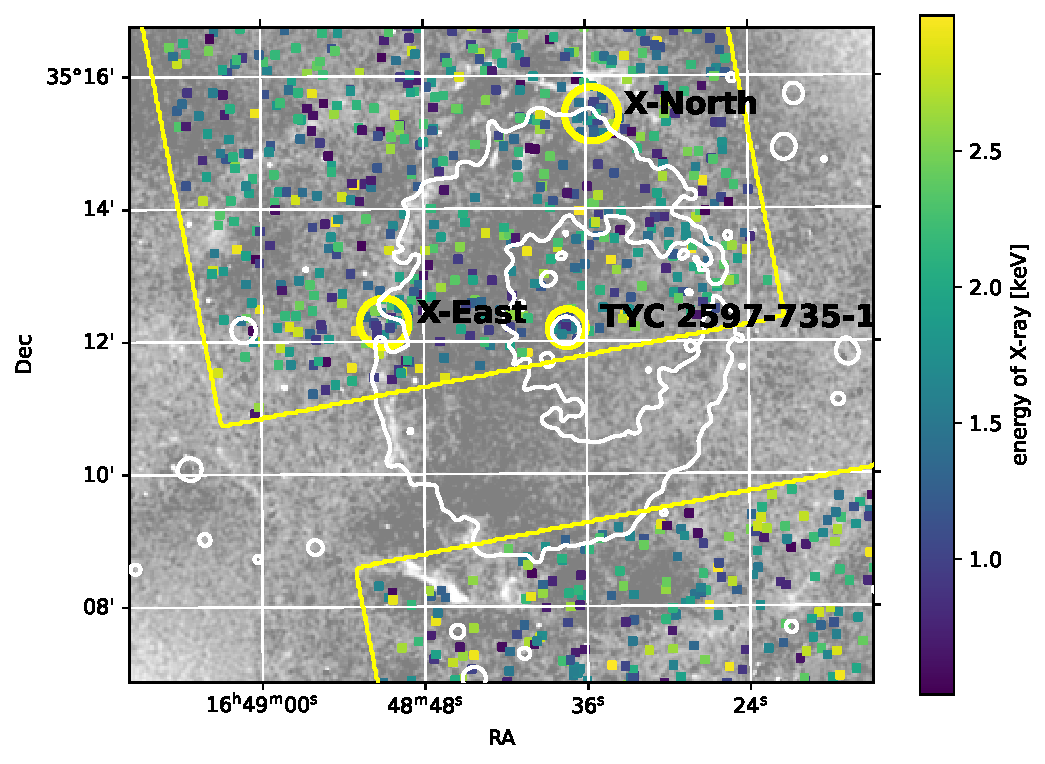
\includegraphics[width=\textwidth]{figures/chandraimage.pdf}
    \caption{X-ray emission around TYC 2597-735-1. The greyscale image shows H$\alpha$ emission and the white contours outline the UV emission. Data for both is taken from \citet{2020Natur.587..387H}, see there for details. The colored squares mark the position of individual X-ray photons, where the color denotes the energy of each particular photon. Only photons in the energy range given on the color bar are shown. Yellow circles mark the position of the three detected sources and their 90\% PSF size, which we use as the extraction region to extract spectra. The thin yellow lines outlines the area covered by Chandra in the observation.}
    \label{fig:chandraimage}
\end{figure*}

\subsection{Source detection}
We expect any emission from the outflows to be soft (section~\ref{sec:outflow}), but absorbed due to the large distance of TYC 2597-735-1. To reduce the high-energy background, which can overwhelm weak, soft sources, we construct a narrow band image in the 1-2~keV range
and run a source detection with the CIAO \texttt{wavdetect} task, which convolves the input image with a wavelet, taking the size of the PSF at that image location into account. We bin up the image such that it contains $2.6\times10^4$ pixels in Chandra's field-of-view and set the significance threshold such that we expect no more than one false detection in $10^5$~pixels. That way, any source detected by \texttt{wavdetect} is likely to be real. We find three sources (table~\ref{tab:src}), all of which coincide with UV/optical emission features. All three sources have similar count rates and similar PSF sizes and thus similar positional uncertainties of about 2\arcsec{}.

\begin{table}
\caption{Detected X-ray sources\label{tab:src}}
\begin{tabular}{ccccccc}
\hline \hline
name & RA & DEC & $\sigma_\mathrm{RA}$ & $\sigma_\mathrm{DEC}$ & NET COUNTS & BKG COUNTS\\
 &  &  & $\mathrm{{}^{\prime\prime}}$ & $\mathrm{{}^{\prime\prime}}$ & $\mathrm{ct}$ & $\mathrm{ct}$ \\
\hline
TYC 2597-735-1 & $16^\mathrm{h}48^\mathrm{m}38^\mathrm{s}$ & $35^\circ12{}^\prime11{}^{\prime\prime}$ & 3.2 & 2.0 & $7.5 \pm 3.0$ & $1.52 \pm 0.01 $\\
X-East & $16^\mathrm{h}48^\mathrm{m}50^\mathrm{s}$ & $35^\circ12{}^\prime28{}^{\prime\prime}$ & 2.2 & 2.6 & $3.9 \pm 2.2$ & $1.08 \pm 0.01 $\\
X-North & $16^\mathrm{h}48^\mathrm{m}35^\mathrm{s}$ & $35^\circ15{}^\prime34{}^{\prime\prime}$ & 2.8 & 3.2 & $6.0 \pm 2.8$ & $1.96 \pm 0.02$ \\
\hline
\end{tabular}
\end{table}


We detect a source at the location of TYC 2597-735-1 with (in our narrow band image) $9\pm3$ counts on a background of $1.52\pm0.01$ counts. (The background is known to a high precision because \texttt{wavdetect} determines it over a large area.) Additionally, the probability that any one source randomly overlaps with the known position of TYC 2597-735-1 within the 90\% PSF radius (0.28 arcmin for an energy of 1.5~keV and at the position of TYC 2597-735-1) is only 0.2\%. Thus, we regard this as a highly reliable detection of X-ray emission from TYC 2597-735-1, albeit with large uncertainties on flux and spectral properties due to the small number of counts.

We do detect two other features that are both located just inside the ring of H$\alpha$, one of them is almost due North of TYC 2597-735-1, and the other one to the East (Fig.~\ref{fig:chandraimage}, see table~\ref{tab:src} for source properties).  Neither the GAIA DR2 \citep{2016A&A...595A...1G,2018A&A...616A...1G} nor the 2MASS \citep{2006AJ....131.1163S} catalog show any point sources coinciding with these features; thus the X-ray emission cannot be caused by a foreground star. Together with the soft X-ray spectrum (see below) this also rules out most classes of X-ray background objects. Again, the fact that both features are located at a physically meaningful position between the UV emission (white contour Fig.~\ref{fig:chandraimage}) and the bright H$\alpha$ ring (background image in Fig.~\ref{fig:chandraimage}) argues that these are not background fluctuations, but probably very weak sources that are physically associated with the outflow. However, the number of detected photons is low and only deeper X-ray observations will be able to unambiguously confirm these detections.

Given the low number of counts and the size of the Chandra PSF that far away from the aimpoint, all three sources are compatible with point sources, but we expect that the latter two sources are probably spatially extended just like the H$\alpha$ and the UV emission is. However, the low count number does not allow us to actually fit the source shape or extent, so we treat them like point sources below.

We also search for extended emission on larger scales that coincide with either the FUV emission (using a region bounded by the white contours  in Fig.~\ref{fig:chandraimage}) or a region FUV and H$\alpha$, i.e.\ a ring on the outside of the white contour in Fig.~\ref{fig:chandraimage} that contains the sources labelled ``X-North'' and ``X-East''. The latter might be a sign of a shocked, X-ray emitting region in front of the FUV emission. However, we do not know a-priory which level of contour lines might be correlated, so the selection of the region is somewhat arbitrary. We do not see significantly enhanced emission --except for the three point-like sources discussed above-- compared to a background region on the northern half of the chip. To obtain an order-of-magnitude estimate how bright an extended source would have to be for a secure detection, we take the $3\sigma$ uncertainty of the observed background flux (about $10^{-5}$~counts~s$^{-1}$~arcsec$^{-2}$) in the same 1-2~keV energy range as for the source detection above and convert that the number into an energy flux per surface area in the plane of the sky. We find that emission would have to be stronger than a few times $10^{31}$~erg~s$^{-1}$~pc$^{-2}$ in this band to be detected significantly above the background.

\subsection{Source properties}
For all three regions, the detected soft photons are distributed over the observing time; we do not see strong clustering that would indicate a large flare, but given the low count numbers, variability with factors of a few cannot be excluded.

For low count numbers, a formal spectral fit does not provide very reliable results; \citet{2010ApJ...708.1760G} instead provide a non-parametric method to estimate X-ray properties of a source based on the median energy. Their method is validated through extensive simulations and comparison with about 2000 faint stellar source observed with Chandra/ACIS; it essentially relies on the fact that photons in the hard band are not affected by the absorbing column density $N_\mathrm{H}$, so the median energy in the hard band can be used to estimate the plasma temperature. With that fixed, the soft band flux can provide an estimate of $N_\mathrm{H}$. Without hard flux, as in our case, there is a fundamental degeneracy affecting any parameter estimation method: A cool, but bright plasma with a high $N_\mathrm{H}$ produces a spectrum very similar to the spectrum emitted from a hotter, but less absorbed plasma.

We use both the \citet{2010ApJ...708.1760G} method and spectral fitting to estimate the parameters of TYC 2597-735-1 and the two emitting regions located close to the H$\alpha$ ring, where we combine the spectra of the latter two regions, since the count number is very low and X-ray properties (see the color of the detected photons in Fig.~\ref{fig:chandraimage}) and location (between H$\alpha$ ring and UV emission) are very similar.

We extract spectra for all three sources using circular extraction regions that encompass 90\% of the PSF at 1.5~keV at the location of the source. A background spectrum is extracted from a large region on the same chip, that is located outside of the UV contours shown in Fig~\ref{fig:chandraimage}. Below 7~keV, the background is well described by a flat component, except for a significant feature around 2.2~keV. Therefore, we exclude the regions 2.0-2.5~keV and $>7.0$~keV from fitting. We then simultaneously fit the source and background spectra using a modified Cash statistic \citep{1979ApJ...228..939C} as implemented in Sherpa \citep{2007ASPC..376..543D,doug_burke_2021_4428938}. To fit source emission, we use a model of an absorbed, collisionally-excited plasma \citep[APEC model,][]{2012ApJ...756..128F} and add the flat background model, scaled for the different extraction regions. That way, we avoid subtracting the background and retain Poisson statistics. All fits are done on unbinned data, but the spectra are shown binned for display in Figs.~\ref{fig:TYC_spec} and \ref{fig:combined}.

The spectrum for TYC 2597-735-1 is shown in Fig.~\ref{fig:TYC_spec}. We fit $N_\mathrm{H}=(6\pm5)\times10^{21}$~cm$^{-2}$ and a plasma temperature in the range .1-1.5~keV, where the low end of the range requires very large values of $N_\mathrm{H}$ and emission measure. For temperatures around 1~keV, common for stellar sources, the unabsorbed flux is of order $10^{-13}$~erg~s$^{-1}$~cm$^{-2}$, which corresponds to $3\times 10^{30}$~erg~s$^{-1}$ with uncertainties of a factor a few. The non-parametric method finds $N_\mathrm{H}$ around $1\times10^{22}$~cm$^{-2}$ and points to a stellar model with an intrinsic plasma temperature of 0.8~keV, leading to similar total fluxes.
\begin{figure}
    \centering
    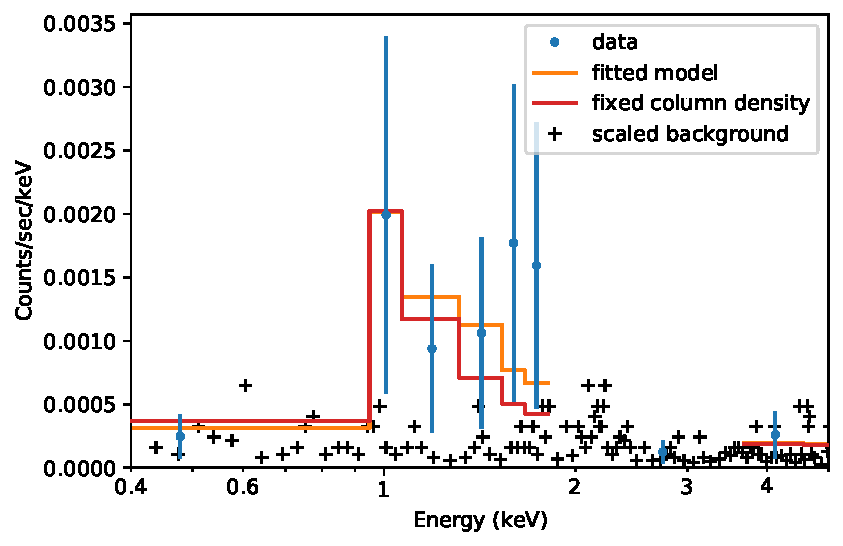
\includegraphics[width=\textwidth]{figures/TYC_spec.pdf}
    \caption{Spectrum of TYC 2597-735-1 binned to two count per bin. Error bars are just to guide the eye. The orange line shows the best fit model discussed in the text. Green crosses show the background rate, scaled from a much larger area. The background feature that caused us to ignore the region 2.0-2.5~keV in the fit is also visible. Error bars on the background are omitted for clarity.
    \label{fig:TYC_spec}}
\end{figure}

The combined spectrum for the other two emission regions is shown in Fig.~\ref{fig:combined}. We fit $N_\mathrm{H}=(1.3_{-0.6}^{+2})\times10^{22}$~cm$^{-2}$ and a plasma temperature of $0.5_{-0.3}^{+\infty}$~keV. For temperatures around 0.5~keV, which we will argue are physically reasonable in Sect~\ref{sec:outflow}, the unabsorbed flux is of order $3 \times 10^{-13}$~erg~s$^{-1}$~cm$^{-2}$, which corresponds to $10^{31}$~erg~s$^{-1}$ with uncertainties of a factor a few. We do not apply the non-parametric method, since this is not a stellar source.
\begin{figure}
    \centering
    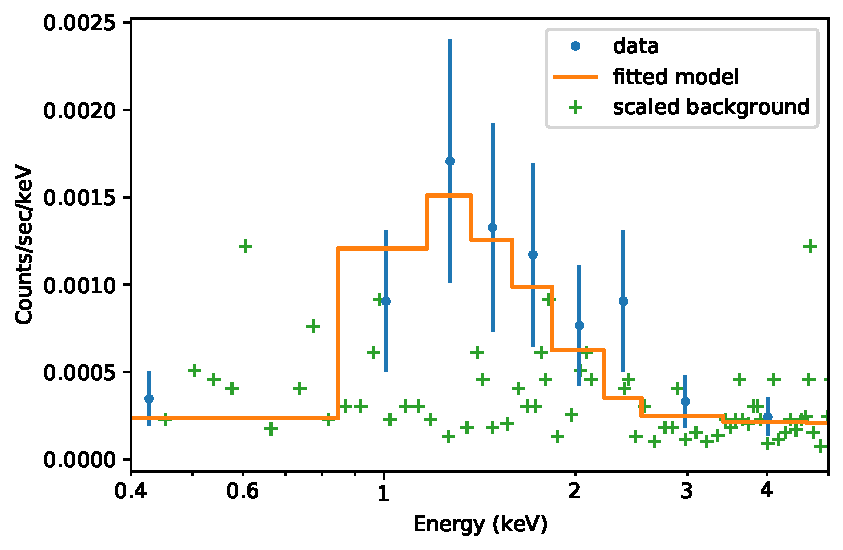
\includegraphics[width=\textwidth]{figures/combined.pdf}
    \caption{Combined spectrum from the two X-ray detected regions in the outflow. See Fig.~\ref{fig:TYC_spec} for an explanation of symbols.
    \label{fig:combined}}
\end{figure}


\subsection{Optical photometry}
The Transiting Exoplanet Survey Satellite (TESS; \citealt{Ricker2015}) observed TYC 2597-735-1 in its sector 25 and camera 1 from 2020-May-13 until 2020-Jun-08.
TESS is an optical photometry mission with four 24x24 degree cameras operating in the 600-1000\,nm range. The spacecraft scans through the entire sky in sectors of $\sim28$\,day duration, whereby each sector is divided into two satellite orbits of $\sim14$\,day duration.
We identified TYC 2597-735-1 as TIC 284856863 in the TESS Input Catalog version 8 \citep{Stassun2019} and found that it fell into TESS's full-frame images with 30 min cadence.
We retrieved the mission's official MIT quick-look-pipeline (QLP) light curve from the High-Level Science Products (HLSP) via the Mikulski Archive for Space Telescopes (MAST) archive.

Inspecting the detrended light curve and corresponding background flux, we found significant variability (Fig.~\ref{fig:TESS_light_curve}).
This could be due to either intrinsic stellar variability or instrument systematics, or a combination of both.
On the one hand, the rotation period of TYC 2597-735-1 is at least 13.75 days, a lower limit derived from the $v \sin{i}$ measurements \cite{???}. This would match the period of the two major brightness increases towards the ends of each TESS orbit (TJD 1,990-1,995 and 2,005-2,010; where TJD = $\mathrm{BJD_{TDB}}$ - 2,457,000).

On the other hand, the TESS data release notes\footnote{\url{https://tasoc.dk/docs/release_notes/tess_sector_25_drn36_v02.pdf}} state that Earth's scattered light particularly affected this sector and camera. These notes, along with our inspection of the local background flux (Fig.~\ref{fig:TESS_light_curve}) and neighboring stars of similar brightness (not shown here), suggest that these systematics affected mainly the beginnings of each orbit. This means the ends of each orbit should remain reliable.

However, the similarity of the expected stellar rotation period and the TESS orbit duration (both $\sim14$\,days) make it difficult to disentangle the true origin of the variability. TESS will re-observe TYC 2597-735-1 in sectors 51 and 52 (from 2022-Apr-22 until 2022-Jun-13). This extended observing window, the possibility of increased observation cadence (2\,min or even 20\,s cadence) and improved visibility will help to understand TYC 2597-735-1's behavior at optical wavelengths.

\begin{figure}
    \centering
    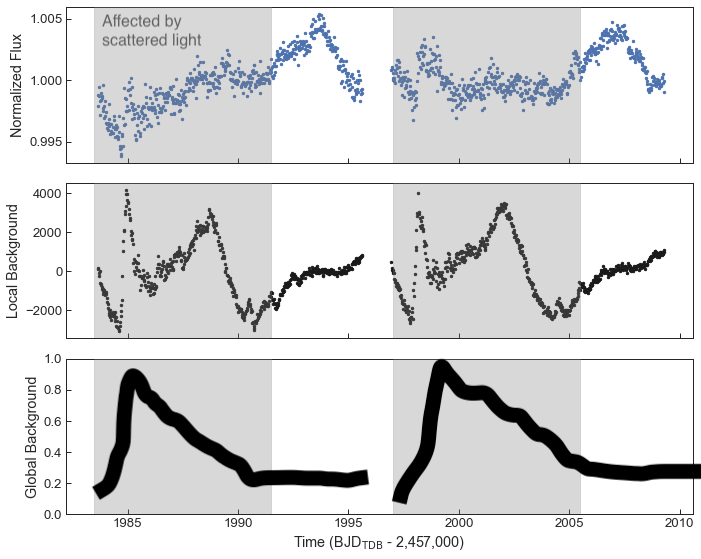
\includegraphics[width=0.8\textwidth]{figures/TESS_light_curve.png}
    \caption{\textcolor{red}{THIS IS JUST A PLACEHOLDER.} The TESS light curve, local background, and global background for TYC 2597-735-1. The observations taken in sector 25 with camera 1 range from 2020-May-13 until 2020-Jun-08. The light curve has been corrected for background effects and displays significant variability. While the beginnings of each TESS orbit suffer from systematics caused by Earth's scattered light (grey-shaded areas), the ends of the orbit show brightness increases that could be of astrophysical nature.
    \label{fig:TESS_light_curve}}
\end{figure}

\cite{2020Natur.587..387H} noticed an RMS scatter around 0.008~mag --significantly larger than the formal uncertainties-- between runs of ground-based $B$ band observations between 2015 and 2019. They attributed this to systematic calibration uncertainties. However, given the variability in the TESS lightcurve on a similar level, this might instead be a signature of stellar activity.

TBD: Get level of activity in B band for similar stars? Maybe in dicussion?


\section{Discussion}  \label{sec:discussion}
Most X-rays from stellar sources originate from optically thin, collisionally excited gas with temperatures of a few MK. The gas can either the heated by magnetic reconnection as in the solar corona, or in shocks (accretion shocks or shocks in winds or jets). Unless the density is very low ($<10^5$~cm$^{-3}$ or so), we can assume that the plasma is in an equilibrium ionization state \citep[see, e.g. the accretion shock simulations in ][]{2007A&A...466.1111G}.

\subsection{X-rays from shocks}
Shocks convert bulk kinetic energy into thermal energy. Possible scenarios here are an accretion shock where material falls from the disk onto the star with close to free-fall velocity, or shocks in outflows. The latter might be seen in different locations: When the outflow runs into the (almost) stationary ISM (forward-shock), the front of the outflowing material is decelerated, which also causes a reverse shock. Last, changes of the outflow velocity over time can lead to internal working surfaces that travel along the flow as faster material catches up with previous slower ejecta.

Assume material of pre-shock density $n_{\rm pre}$ is moving with velocity $v_{\rm pre}$ into a stationary external medium (the ISM in the case of an outflow termination shock or the stellar photosphere in the case of an accretion shock) of particle density $n_{\rm ext}$.  The velocity of the forward shock in the lab frame is given by the shock jump conditions (for adiabatic index $\gamma = 5/3$),
\be
v_{\rm fsh} = \frac{4}{3}v_{\rm psh}, \label{eqn:vsh1}
\ee
where $v_{\rm psh}$ is the velocity of the post-shock gas.  The reverse shock velocity (also in the lab frame) is given by
\be
v_{\rm rsh} \simeq \frac{4}{3}v_{\rm psh} - \frac{v_{\rm ej}}{3}
\label{eqn:vsh2}
\ee

From the jump conditions, the shocks will heat gas to a temperature
\be
kT_{\rm sh} \simeq \frac{3}{16}\mu m_p v_{\rm sh}^{2} \approx 0.3\,{\rm keV}\left(\frac{v_{\rm sh}}{500\,{\rm km/s}}\right)^{2},
\label{eqn:Tshock}
\ee
where we have taken $\mu \simeq 0.62$ for fully ionized solar composition gas.  Here $v_{\rm sh}$ is the shock velocity relative to the upstream rest frame.

\subsection{TYC 2597-735-1}
There are a variety of physical mechanisms that may be responsible for the X-ray emission observed at TYC 2597-735-1. The point of interest is that TYC 2597-735-1 is strongly suspected of undergoing a merger event with a smaller, $\sim$0.1 M$_{\odot}$ companion $\lesssim$5,000 years ago \citep{2020Natur.587..387H}. Such a collision and subsequent engulfment of a stellar companion would disrupt the equilibrium state of the surviving star, potentially leading to enlarged surface convective zone regions (e.g., \citealt{}), accretion flows from surrounding circumstellar material that continue to disturb the star's outermost surface regions (e.g., \citealt{}), and sustained outflows that continue to eject material from the system (e.g., \citealt{Zuckerman+2008}). Here, we explore different mechanisms that may be responsible for the X-ray emission observed at TYC 2597-735-1.


\subsubsection{X-rays from Accretion Shocks onto TYC 2597-735-1}

Current observations suggest TYC 2597-735-1 harbors a substantial circumstellar disk, which may have an inner rim as close as $\sim$0.1 AU \citep{2020Natur.587..387H}. Much like planet-forming accretion disks, complex interactions between these disks and stars via magnetospheric accretion can lead to matter falling onto the star, potentially generating X-rays at free-fall shock regions \citep[e.g.]{2007A&A...466.1111G}. Here, we explore whether this accretion shock near TYC 2597-735-1 provides the right conditions to generate the observed $L_{\rm X}$ and subsequent 1-2 keV photons.

With the stellar parameters from table~\ref{tab:parameters} we calculate the free fall velocity of material onto TYC 2597-735-1 as
\begin{equation}
    v_{\rm ff} = \left( \frac{2 G M_{\star}}{R_{\star}} \right)^{1/2} \left( 1 - \frac{R_{\star}}{R_{\rm M}} \right)^{1/2} \approx 280 \left( \frac{M_{\star}}{0.5 M_{\odot}} \right)^{1/2} \left( \frac{R_{\star}}{2 R_{\odot}} \right)^{-1/2} km/s,
\end{equation}
or $v_{\rm ff} \lesssim$ 260 km/s. At this free fall velocity, the temperature of the shocked material according to eqn~\ref{eqn:Tshock} is $\lesssim$ 775,000 K -- too low to explained the observed X-ray flux.
Instead, the accretion shock should peak in luminosity in the EUV ($\sim$180 - 280 {\AA}) where the total shock luminosity is expected to be a small fraction of $L_{\star}$:
\begin{equation}
    L_{\rm sh} = \frac{1}{2} \dot{M} v_{\rm ff}^{2} \approx 3.5 \times 10^{-3} L_{\odot},
\end{equation}
or $L_{\rm sh}/L_{\rm bol} <$ 3$\times$10$^{-5}$.

\subsubsection{Shocks at the base of the outflow}
In the young star DG~Tau, X-rays have been observed at the base of the outflow \citep{2008A&A...488L..13S} possibly related to the launching or collimation \citep[e.g.]{2014ApJ...795...51G,2018A&A...615A.124U}. In DG~Tau, the soft X-ray emission is offset by about 40~au, but given the source location offset from \emph{Chandra}'s optical axis, the distance of TYC 2597-735-1, and the viewing geometry where the outflow axis is close to the line-of-sight, we do not expect a positional offset here.

If we assume that a fraction $\eta_{\rm j} \sim 10\%$ of the accreted matter is launched into a bipolar collimated outflow (``jet'') with an outflow velocity $v_{\rm j}$ some multiple $\sim 3$ of the surface escape speed of TYC, $\approx (GM_{\star}/R_{\star})^{1/2} \approx 160$ km s$^{-1}$, then the present-day jet power is given by
\be
L_{\rm j} \approx \frac{1}{2}\eta_{\rm j}\dot{M}_{\star}v_{\rm j}^{2} \approx 5\times 10^{32}\,{\rm erg\,s^{-1}}\,\left(\frac{\eta_{\rm j}}{0.1}\right)\left(\frac{\dot{M}_{\star}}{10^{-7}M_{\odot}\,\rm yr^{-1}}\right)\left(\frac{v_{\rm w}}{400\,{\rm km\,s^{-1}}}\right)^{2},
\label{eqn:jetpower}
\ee
This is in principle sufficient to explain the X-ray point source overlapping TYC, $L_{\rm X} \sim 10^{31}$ erg s$^{-1}$. To match the temperature of the X-rays, we need internal shocks of order 500~km~s$^{-1}$ (eqn.~\ref{eqn:Tshock})
for instance as a result of the wind velocity increasing with time due to the radial contraction of TYC (and hence increase of the escape speed from the inner edge of the accretion disk) as the star undergoes thermal-timescale contraction following the merger \citep[][extended Figure 7]{2020Natur.587..387H}. In young stars, outflows often have different velocity components, where only the fastest and innermost components shock to produce X-rays, while most of the mass in seen in slower components. For example, in DG~Tau, the measured velocity in the UV is similar to the outflow velocity of the BRN. However, such a scenario would require an unreasonably large mass-loss, since eqn.~\ref{eqn:jetpower} already requires that 10\% of the total accretion rate shocks to produce X-rays. The entire outflow would have to be accelerated to $\sim 900$~km~s$^{-1}$ (several times the escape speed), and pass through a shock front with $\Delta v=500$~km~s$^{-1}$, to produce sufficient luminosity at X-ray emitting temperatures and continue the outflow with the velocity of $\sim 400$~km~s$^{-1}$ observed in the BRN. We cannot rule out this scenario, but the high launching speed and the fact that it does not explain the variability in the TESS and RV lightcurves make it unlikely that shock at the base of the outflow are the main component of the observed X-ray emission.


\textcolor{blue}{HMG: I'm not convinced that the scenario above is realistic. The entire mass outflow would have to be 900 km/s fast (500 for the shock and 400 because we see flow velocity in the BRN after). Thus, I commented out Brian's section on N\_H for such a scenario. We can bring it back in, if you disagree!}
%If the jet is conical in shape and subtends a fraction $f_{\Omega} < 1$ of the total $4\pi$ solid angle, then the radial density profile of the jet is approximately given by
%\begin{eqnarray}
%n_{\rm j} &\approx& \frac{\eta_{\rm j}\dot{M}_{\star}}{4\pi f_{\Omega}m_p v_{\rm j} r^{2}} \nonumber \\
%&\approx& 8\times 10^{-4}\,{\rm cm^{-2}}\left(\frac{\eta_{\rm j}}{0.1}\right)\left(\frac{f_{\Omega}}{0.1}\right)^{-1}\left(\frac{\dot{M}_{\star}}{10^{-7}M_{\odot}\,\rm yr^{-1}}\right)\left(\frac{v_{\rm j}}{400\,{\rm km\,s^{-1}}}\right)^{-1}\left(\frac{r}{1\,{\rm pc}}\right)^{-2},
%\end{eqnarray}
%while the column density external to some radius $r$ is given by
%\begin{eqnarray}
%N_{\rm H} \approx \int_{r}^{\infty} n_{\rm j}dr &=& \frac{\eta_{\rm j}\dot{M}_{\star}}{4\pi f_{\Omega}m_p v_{\rm j} r} \nonumber \\
% &\approx& 2\times 10^{15}\,{\rm cm^{-2}} \left(\frac{\eta_{\rm j}}{0.1}\right)\left(\frac{f_{\Omega}}{0.1}\right)^{-1}\left(\frac{\dot{M}_{\star}}{10^{-7}M_{\odot}\,\rm yr^{-1}}\right)\left(\frac{v_{\rm j}}{400\,{\rm km\,s^{-1}}}\right)^{-1}\left(\frac{r}{1\,{\rm pc}}\right)^{-1},
%\label{eq:NHjet}
%\end{eqnarray}
%where $m_p$ is the proton mass and we have normalized $r$ to a maximum radius corresponding to outer extent of the BRN.

%Equation (\ref{eq:NHjet}) shows that, in principle, jetted X-ray emission could originate from radii as small as $\sim 10^{-6}$ pc (corresponding to $\sim 10^{-4}$ arcsec projected angular offset from TYC) and not overproduce the $N_{\rm H} \approx 10^{21}-10^{22}$ cm$^{-1}$ values of the X-ray source.  At this radius, the density could be as high as $n_{\rm j}(10^{-4}{\rm pc}) \sim 10^{7}{\rm cm^{-3}},$ more than sufficient for any shocks in the outflow to be radiative (i.e., to cool through UV/X-ray emission faster than the radial expansion time) and hence to tap into a sizable fraction of the jet power, $L_{\rm j}$, to power the observed X-ray emission.


\subsubsection{Star Dynamo Generated X-rays}
% From emails:
% Ken - 07/09
% Okay, FINALLY got to re-running some models and looking at the time evolution of the Rossby number.  This is for the 0.1 Msol companion merging when the primary has a radius of 5 Rsol (i.e. the model that best fit the observations in the extended data Figure 7 of the 2020 paper).  It has two convection zones up through >5000 yr: one deep one (r ~ 0.5 Rsol) where the planet disrupted, and a surface one.  I'm just quoting values for the surface convection zone.
%Time [yr]     dr of conv zone [cm]     Max v_conv in zone [cm/s]   dr/vconv [d]
%100             7.74e9                           1.33e6                                0.0673
%200             5.34e9                           1.23e6                                0.0503
% 500             5.81e9                           1.05e6                                0.0642
% 1000           2.12e10                         7.85e5                                0.312
% 2000           4.24e10                         5.59e5                                0.877
% 5000           7.63e10                         3.41e5                                2.589

% So the Rossby number (assuming P_rot = 20 d) does start climbing, which is I think is what's necessary to explain the X-ray luminosity, but I don't think it's high enough by 1000 yr.

% Other models might match better...  Also, these are all for a mass of 2.2 Msol, which is probably not right anyway.
%
% Keri - 07/12
% Ken's models are consistent with Brian's estimates (Cx ~ 1.0e-4), so we can tweek Brian's numbers by the factors from the models and the results should be the same. The early time overturn timescale (t<2,000 years) produces too high a Rossby number to create magnetic activity (like Ken said), unless the rotation period of this star was much higher in the past. I don't know how we might estimate that, though.

% My suggestion is that we can create a table with the convection properties over time from the models, provided by Ken below (I can do this). From that, we can show that we don't expect the surface convection zone properties to be sufficient to lead to detectable levels of magnetic activity, as the Rossby number was probably too high up until t~5,000 years (with the caveat of the rotation period of the surface, which is not known)(unless Ken's models also tell us that?). At t~5,000 years, the Rossby number falls into the regime where it could lead to magnetic activity, and it is on order what Brian already reported: higher than nominal MS and giant stars, but lower than pre-MS stars (which tend to be in the saturated zone, Cx ~ 1.0e-3).
%
The measure by which the level of magnetic activity for pre-main sequence, main sequence, and giant stars has often been invoked is a star's Rossby number \citep{Preibisch+2005, Pizzolato+2003, Gondoin+2005}.
The Rossby number, which is the ratio of convective overturn velocity to rotational period, i.e.

\begin{equation}
{\rm Ro} \sim \frac{P_{\rm rot}}{\tau_{\rm conv}},
\end{equation}

has notable correlations with main sequence stellar magnetic activity and is well established in the frame of stellar dynamo models (e.g., \citealt{Brandenburg+1998}).

\citet{2020Natur.587..387H} used a series of \texttt{MESA} models to simultaneously track the temporal behavior of a recent stellar merger to match its properties to observed characteristics of TYC 2597-735-1 and estimate the original binary star properties (in particular, M$_{\star}$) that best matches the anticipated age (from the expansion rate of the BRN) and observed properties of TYC 2597-735-1 today. Using the best-fit model output from \citet{2002ApJ...576L.149R}, we extract the properties of possible convection zones that may have arisen in TYC 2597-735-1 post-merger with a 0.1 M$_{\odot}$ companion. The primary star in the \texttt{MESA} evolutionary model has a mass M$_{\star}$ = 2.17 M$_{\odot}$ and a radius R$_{\star}$ = 5 R$_{\odot}$. The models suggest the primary (surviving) star may have two prominent convection zones that persist $>$5,000 years after the stellar merger: a deep convection zone ($\sim$0.5 R$_{\odot}$), and a surface one. As the dynamo near the stellar surface is the one that likely controls magnetic activity, we focus on the properties of the surface convection zone of our modeled star.

% Table here
\input mesatable.tex


Table~\ref{tab:mesa} presents the total length of the surface convection zone, the velocity of the zone at the bottom of the convective region, and the corresponding overturn time $\tau_{\rm conv}$ at different snapshots in time since $t=0$ of the complete stellar merger in the \citet{2020Natur.587..387H} best-fit \texttt{MESA} model for TYC 2597-735-1. The last column shows the approximate Rossby number of the modeled surface convection zone at each timestamp in the \texttt{MESA} model. Each Rossby number assumes the primary star has a rotation period of 13.75 days \citep{2020Natur.587..387H}, regardless of time since merger.

Taking $\tau_{\rm conv} \sim 4$ d for a 10 $R_{\odot}$ convective star (\citealt{Soker&Tylenda2007}, Eq.~4) and $P_{\rm rot} \sim 20$ d as measured for TYC assuming a rotation axis aligned with the symmetry axis of the BRN \citep{2020Natur.587..387H}, we infer ${\rm Ro} \sim 4$.  This is within the range of magnetic activity, which ceases at ${\rm Ro} \gtrsim 10$ (Pizzolato et al. 2003).   {\bf Ken could estimate $\tau_{\rm conv}$ more accurately using his models specific to TYC...}

The predicted X-ray luminosity from the dynamo is (e.g., Soker \& Tylenda 2007)

\begin{equation}
\frac{L_{\rm X}}{L_{\rm bol}} = C_{\rm x}{\rm Ro}^{-2}
\end{equation}

Thus, taking $L_{\rm bol} = 100L_{\odot}$ for TYC and ${\rm Ro} = 4$, we find that explaining the measured $L_{\rm X} \sim 6\times 10^{30}$ erg s$^{-1}$ requires $C_{\rm x} \sim 2\times 10^{-4}$ for TYC....  This activity level is a factor $\sim 10$ and $\sim 100$ higher than for main sequence (Pizzolato et al. 2003) and giant stars (Gondoin 2005), respectively.  The level of X-ray activity {\it might} be consistent with YSOs, which can achieve ratios $L_{\rm X}/L_{\rm bol}$ up to a factor of 30 times higher than for main sequence stars (Preibisch et al. 2005; see their Fig. 10), possibly as a result of the accretion disk present in these systems (absent in main sequence or ordinary giant stars, but present around TYC...).


\subsection{Large scale outflow}
We now place limits on the properties of the outflow and the BRN using the upper limit for large-scale X-ray emission coincident with the FUV emission and our detection of the point-like sources X-East and X-North.

Assume the BRN ejecta of density $n_{\rm BRN}$ is expanding at $v_{\rm ej} \simeq 400$ km/s into a stationary external medium of particle density $n_{\rm ism}$.  In the limit that the shocked gas is still moving out with the same velocity as the BRN, we get  $v_{\rm psh} \simeq v_{\rm ej}$, $v_{\rm fsh} \simeq (4/3)v_{\rm ej}$, and $v_{\rm rsh} \simeq v_{\rm ej}$ (i.e.\ the reverse shock is not yet making much progress moving back through the ejecta), using eqns~\ref{eqn:vsh1} and \ref{eqn:vsh2}.  However, if, as we expect in the BRN from the bright UV emission, the shock has already swept up considerable gas from the external medium and begun to decelerate, then $v_{\rm fsh} \ll v_{\rm ej}$ and $v_{\rm rsh} \simeq -v_{\rm ej}/3$.

$v_{\rm sh}$ in eqn.~\ref{eqn:Tshock} is the shock velocity relative to the upstream rest frame (i.e. $v_{\rm sh} \simeq v_{\rm fsh}$ in the case of the forward shock with stationary upstream, but $v_{\rm sh} \simeq v_{\rm ej}-v_{\rm rsh}$ in the reverse shock).  From the above, we expect the reverse shock will be strongest, with $v_{\rm sh} \simeq (4/3)v_{\rm ej} \approx 500$ km/s.


\subsubsection{Sources X-East and X-North}
The sources X-East and X-North are compatible with point sources. Given the size of the PSF, we use 1~arcsec ($d_\mathrm{sh}=1900$~au at the distance of TYC 2597-735-1) as upper limit of the source size and 500~km~s$^{-1}$ as the shock velocity for the ejecta, compatible with the observed X-ray spectrum.

\citet{2002ApJ...576L.149R} provide a
semi-analytical formula for the cooling length
$d_{\mathrm{cool}}$ of gas
heated in fast shocks ($\Delta v \ga 200$ km/s) caused by ramming into an obstacle
which we can rewrite as:
\begin{equation}
d_{\mathrm{cool}} \approx 20.9 \mathrm{ AU}
    \left(\frac{10^5\mathrm{ cm}^{-3}}{n_0}\right)
    \left(\frac{v_{\mathrm{shock}}}{500\textnormal{ km s}^{-1}}\right)^{4.5},
\label{raga}
\end{equation}
where $n_0$ is the pre-shock particle number density, equal to a
quarter of the post-shock number density $n$ in the strong shock
approximation.

Since $d_{\mathrm{cool}}$ is much smaller than the size scale of the outflow we can neglect spherical expansion over the thickness of the shock.
To fit such a shock into 1900~au, the density must be $>10^3\mathrm{ cm}^{-3}$. The emission spectra calculated by \citet{2002ApJ...576L.149R} include both continuum and line emission in the X-ray band. According to their equations 8 and 9, a non-radiative shock with $n_0=10^3\mathrm{ cm}^{-3}$ and a diameter equal to the size of the PSF emits just enough flux to explain the X-ray emission from either X-North or X-East. Such a shock would have a mass flux of $\dot M = \mu m_\mathrm{p} n_0 v_\mathrm{sh} \pi (d_\mathrm{sh}/2)^2 \sim 10^{-8}\;M_\sun\;\mathrm{yr}^{-1}$.
Should the densities by higher, both the cooling length and the volume of the shock would be smaller, but the mass flux stays unchanged.

\citet{2020Natur.587..387H} estimate the total mass (of neutral hydrogen) of the BRN to $<0.008\;M_\sun{}$. If the mass of the BRN was ejected over the course of 1000~yr, the mass flux is $10^{-5}\;M_\sun\;\mathrm{yr}^{-1}$. The two regions X-North and X-East together cover only a small fraction of the total area of the BRN (Fig.~\ref{fig:chandraimage}), but it is conceivable that 0.1\% of the total mass flux of the BRN outflow is concentrated at these locations. In order to generate X-rays here but not in other parts of the BRN, some special condition must trigger a stronger shock here, such as a pre-existing clump in the ISM which serves as obstacle for the shock. X-North and X-East are located just on the outside of the FUV emission on the ring of the H$\alpha$ line, so the ISM may be be cleared in these locations yet. Similarly, the initial outflow could be clumpy and inhomogeneous in density and velocity and X-North and X-East represent two locations where such dense clumps are colliding; if that is the case, then X-ray sources may flicker on and off all around the ring over a time scale of $<20$~yr (gas at 500~km~s$^{-1}$ needs 20 years to pass through a cooling zone of $d_{\mathrm{cool}}=2000$~au). This hypothesis is testable with new observations!
The H$\alpha$ emission ring also shows some clumpiness on the outside of the BRN. On the other hand, the UV emission from the BRN itself is remarkably smooth, even when taking into account the larger PSF of \emph{GALEX} ($FWHM \sim 5$~arcsec) compared to the H$\alpha$ observations.


\subsubsection{Shock Interaction with the ISM}

Assume the BRN shocks cover a fraction $f_{\Omega} \simeq 0.3$ of the total 4$\pi$ solid angle.  The volume of the hot gas behind the shock is therefore $V_{\rm X} \simeq \frac{R_{\rm BRN}}{4}(4\pi f_{\Omega} R_{\rm BRN}^{3}) \simeq 2\times 10^{56}$ cm$^{-3}$, where we have taken $R_{\rm BRN} \approx 6\times 10^{18}$ cm as the BRN radius, and $R_{\rm BRN}/4$ is the radial thickness of the post-shock gas given its compression by a factor of 4 for a $\gamma = 5/3$ shock.

The X-ray spectrum will be a combination of emission from collisionally excited lines and free-free emission and for low densities the plasma may not be in thermal ionization equilibrium after the shock. As an estimate, we continue looking at the free-free emission only.

The total X-ray luminosity is given by
\be
L_{\rm X} \simeq j_{\nu}(T_{\rm sh},n_{\rm sh} = 4 n)V_{\rm X},
\ee
where the free-free emissivity of solar-metallicity gas,
\be
j_{\nu} \approx 2\times 10^{-27}T^{1/2}n_{\rm sh}^{2}\bar{g}\,{\rm erg\,s^{-1}\,cm^{-3}},
\ee
$n_{\rm sh}$ is the density of the shocked gas, $n$ is the density of the upstream gas, and $\bar{g} \approx 1.2$ is the Gaunt factor.

Combining, we find
\be
L_{\rm X} \approx 1.2\times 10^{34}\,{\rm erg/s}\left(\frac{n}{1\,{\rm cm^{-3}}}\right)^{2}\left(\frac{v_{\rm sh}}{500{\rm km/s}}\right)
\ee
Now, due to the nature of the free-free emission spectrum, the $\nu L_{\nu}$ luminosity in a band $E_X \gtrsim kT$ will be smaller than $L_{\rm X}$ by a factor of $(E_X/kT_{\rm sh})\exp(-E_X/kT_{\rm sh}) \sim 10^{-2}$, where the final numerical estimate assumes $E_X = 2$ keV and $kT_{\rm sh} \sim 0.3$ keV ($v_{\rm sh} \approx 500$ km/s).  Thus, we have
\be
L_{\rm E_X > 1 keV} \sim 10^{-2}L_{\rm X} \sim 10^{32}\,{\rm erg\,s^{-1}}\left(\frac{n}{1\,{\rm cm^{-3}}}\right)^{2},
\ee
however depending sensitively on $kT_{\rm sh}$ (and hence $v_{\rm sh}$).  Thus, given a limit $L_{\rm E_X > 1 keV}  < 6\times 10^{30}$ erg s$^{-1}$, we can put an upper limit of $n < 0.2$ cm$^{-3}$ on the upstream density.

This in turn places a limit on the amount of mass in the BRN (or mass of swept-up ISM in cases when the forward shock dominates),
\be
M_{\rm swept} \sim n m_p V_{\rm X} \sim 0.03M_{\odot} \sim 30M_{\rm J},
\ee
which is consistent with the lower limit of the BRN mass cited in \citet{2020Natur.587..387H} ($M_{\rm BRN} \gtrsim$ 4$M_{\rm J}$).




\subsubsection{Outflow} \label{sec:outflow}
Shock in outflows have been observed in X-ray sources of different evolutionary stage because kinematic energy can be converted into heat in a shock front (Some references either here or in introduction).
Using the strong shock conditions we can transform the thermal energy
k$T$, where k is Boltzmann's constant and $T$ is the temperature, into
the pre-shock velocity in the shock rest frame $v_{\mathrm{shock}}$:
\begin{equation}
\left(\frac{v_{\mathrm{shock}}}{500\textnormal{ km s}^{-1}}\right)^2 \approx
\frac{\textnormal{k}T}{0.33\textnormal{ keV}} \; .
\label{vkt}
\end{equation}
For a travelling shock wave, the pre-shock gas velocity is the sum of $v_{\mathrm{shock}}$ and the motion of the shock front.

Given uncertainty on the fitted value, the observed X-ray temperature if fully consistent with outflow velocities of a few hundred km~s$^{-1}$, that can be deduced from the optical and UV data \citep{2020Natur.587..387H}. The location of the X-ray emission seems to fall slightly inside of the H$\alpha$ emission, but outside of the brightest UV emission (Fig.~\ref{fig:chandraimage}). The interpretation is complicated by the fact that see we both the receding and approaching outflow superimposed on the sky \citep{2020Natur.587..387H}.

\emph{HMG: Could be a shock in front of the UV, as in heated to X-ray temperature and then cools to UV, could be a reverse shock behind halpha}.




\section{Summary and outlook}
\label{sec:summary}

\begin{acknowledgements}
This research has made use of data obtained from the Chandra Data Archive and the Chandra Source Catalog, and software provided by the Chandra X-ray Center (CXC) in the application packages CIAO and Sherpa. This publication makes use of data products from the Two Micron All Sky Survey, which is a joint project of the University of Massachusetts and the Infrared Processing and Analysis Center/California Institute of Technology, funded by the National Aeronautics and Space Administration and the National Science Foundation. We acknowledge the use of TESS High Level Science Products (HLSP) produced by the Quick-Look Pipeline (QLP) at the TESS Science Office at MIT, which are publicly available from the Mikulski Archive for Space Telescopes (MAST). Funding for the TESS mission is provided by NASA's Science Mission directorate.
This work has made use of data from the European Space Agency (ESA) mission {\it Gaia} (\url{https://www.cosmos.esa.int/gaia}), processed by the {\it Gaia} Data Processing and Analysis Consortium (DPAC, \url{https://www.cosmos.esa.int/web/gaia/dpac/consortium}). Funding for the DPAC has been provided by national institutions, in particular the institutions participating in the {\it Gaia} Multilateral Agreement.
HMG was supported by the National Aeronautics and Space Administration through Chandra Award Number GO9-20018X issued by the Chandra X-ray Observatory Center, which is operated by the Smithsonian Astrophysical Observatory for and on behalf of the National Aeronautics Space Administration under contract NAS8-03060.
KH was supported by the David {\&} Ellen Lee Prize Postdoctoral Fellowship in Experimental Physics at Caltech and the National Aeronautics and Space Administration Astrophysics Research and Analysis (APRA) Grant Number 80NSSC20K0395.
MNG acknowledges support from MIT's Kavli Institute as a Juan Carlos Torres Fellow.
\end{acknowledgements}

\facilities{Chandra/ACIS, TESS}

\software{AstroPy \citep{2013A&A...558A..33A,2018AJ....156..123A}, CIAO \citep{2006SPIE.6270E..1VF}, NumPy \citep{van2011numpy,harris2020array}, Matplotlib \citep{Hunter:2007}, Sherpa \citep{2007ASPC..376..543D,doug_burke_2021_4428938}}

\bibliography{bib}{}
\bibliographystyle{aasjournal}

%% This command is needed to show the entire author+affiliation list when
%% the collaboration and author truncation commands are used.  It has to
%% go at the end of the manuscript.
%\allauthors

%% Include this line if you are using the \added, \replaced, \deleted
%% commands to see a summary list of all changes at the end of the article.
%\listofchanges

\end{document}
